\section{Evaluation}

We ran real DNS traces, obtained from the Jung {\it et al.} study,
on a simulated DDNS network
of servers to measure load balancing. We set up a
Chord ring of 1000 nodes and inserted the ring with 
real DNS data. Then performed lookup requests both
from a set of one-day worth of DNS queries, and 
from a hypothetical popular-record lookup situation.

%\includegraphics[angle=270,width=3.5in]{figures/ok.fetch.eps}
\begin{figure}
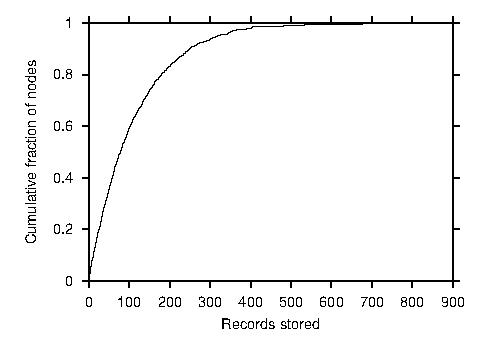
\epsfig{file=figures/ok.store.eps,angle=270,width=3in}
\caption{Cumulative distribution of nodes as a function of number 
of records stored after inserting DNS records from a one-day trace.}
\label{fig:store}
\end{figure}

Figure~\ref{fig:store} shows that half of the nodes
store at most 100 DNS records, and almost all of 
the nodes store at most 400 records. This indicates
DNS servers do not differ much in the amount of work
done in maintaining (storing/replicating) of records.

\begin{figure}
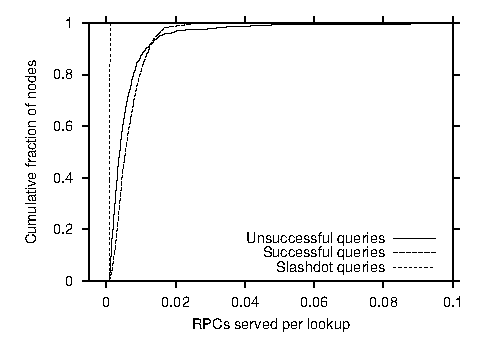
\epsfig{file=figures/both.fetch.eps,angle=270,width=3in}
\caption{Cumulative distribution of nodes as a function of number 
of RPCs served while performing one-day of DNS lookups.}
\label{fig:both-rpc}
\end{figure}

Figure~\ref{fig:both-rpc} shows that 65\% of the nodes
served at most 2000 DNS queries which result in  in one day.

\begin{figure}
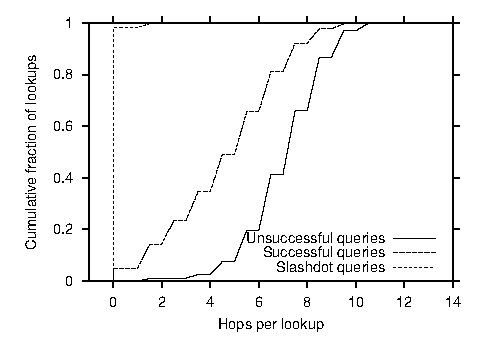
\epsfig{file=figures/hops.eps,angle=270,width=3in}
\caption{Cumulative distribution of nodes as a function of number 
of RPCs served while performing lookups for one very
popular record.}
\label{fig:slashdot-rpc}
\end{figure}

Do a measure of how long it takes to converge to good load 
balancing when there is a burst of lookups for 1 (or more)
popular names. Compare that to the slashdot effects now.

%\subsubsection{Latency}

%We cannot perform a fair measurement of latency so we will do an
%analysis based on counting number of hops between servers
%and combining that with real latency to current root DNS servers.

%XXAdding keys to resource records make them bigger
%XXPublic key cryptography is an expensive operation. 
%DDNS computes pub keys every time.

%DDNS is not going to disappear without an answer for a lookup,
%unlike in the current DNS. So we can't really compare this, but should
%mention about it.
